\graphicspath{{chapters/introduction/figures/}}


\subsection{Motivations}

\begin{frame}{Motivations}
  % \frametitle{Introduction}
  % \framesubtitle{Motivations}
  \begin{block}{\small Statistics}
    \begin{figure}%
      \centering
      \hspace*{\fill}%
      \subfigure[][\tiny \# of cancer cases]{%
        \label{fig:stat1a}%
          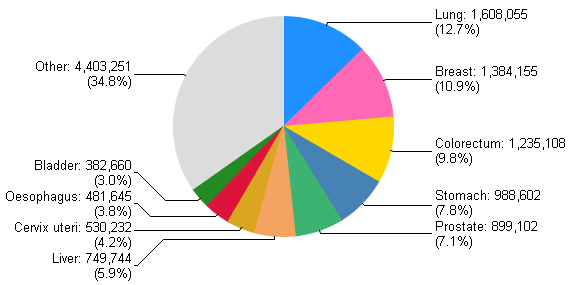
\includegraphics[width=.45\textwidth]{./images/statistics/repartitionCancerIncidence.png}}%
      \hfill%
      \subfigure[][\tiny \# of cancer deaths]{%
        \label{fig:stat1b}%
          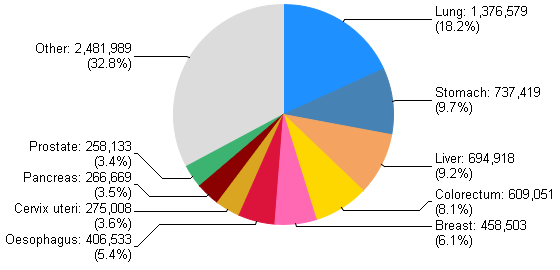
\includegraphics[width=.45\textwidth]{./images/statistics/repartitionCancerDeaths.png}}%
        \hspace*{\fill}%
      \label{fig:stat1}%
    \end{figure}
  \end{block}
  \begin{block}{\small Implications}\footnotesize
    \begin{itemize}
      \item 1.4 million cases per year
      \item 10.9\% of diagnosed cancers
      \item 5\textsuperscript{th} cause of cancer death (1\textsuperscript{th} females)
    \end{itemize}
  \end{block}
\end{frame}

\subsection{Screening}

\begin{frame}{Breast Imaging}
  % \frametitle{Introduction}
  % \framesubtitle{Screening}

    Despite its limitations, Digital Mammography\,(DM) is the main image modality for breast screening. Other image modalities such as Magnetic Resonance Imaging (MRI), Tomography, or Ultra-Sound (US) are being developed. 

    \begin{columns}
      \begin{column}{.6\textwidth}
        \begin{block}{\small Ultra-Sound(US) imaging, advantages:}\footnotesize
          \begin{itemize}
            \item Ability to discern solid lesions typologies
            \item Lesions shielded by dense breast in DM are distinguishable in US
          \end{itemize}
        \end{block}
      \end{column}
      \begin{column}{.4\textwidth}
        \begin{figure}%
          \centering
          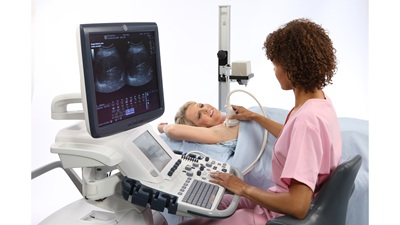
\includegraphics[width=\textwidth]{US_adquisition.jpg}%
        \end{figure}
      \end{column}
    \end{columns}
\end{frame}

\subsection{Image formation, limitations and imaging perspectives}
% \begin{frame}\frametitle{Breast structures under US screening}
% \begin{columns}
% \begin{column}{.48\textwidth}\vspace{-17pt}%\hspace{-1cm}
% \begin{figure}\centering
% \begin{tikzpicture}[scale=.5]
% \begin{scriptsize}
% 	\tikzset{dot/.style={circle,draw=black,inner sep=0mm,minimum size=4pt}}
%     \node[anchor=south west,inner sep=0] at (.2,.2) {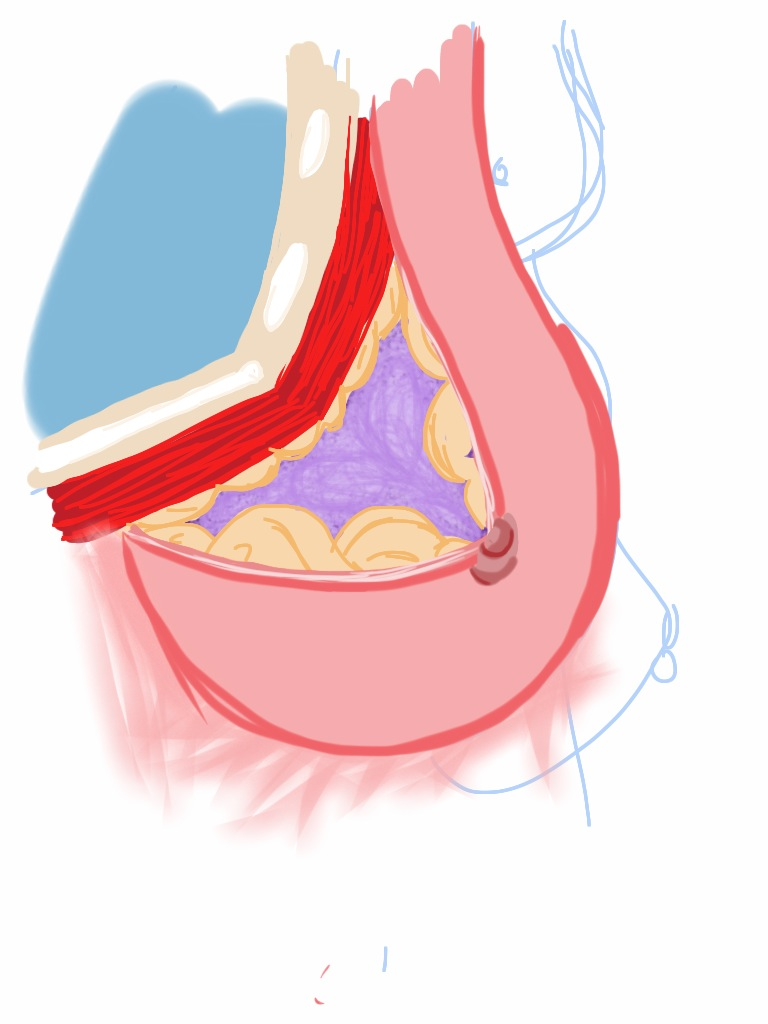
\includegraphics[trim = 20 190 80 20, clip,height=\textwidth]{pit.jpg}};
%     \draw		(1.75,	7.75	) 	node[dot]	(AirCoord)			{}	
%     				(2.5	,	5		) 	node[dot]	(PecCoord)			{}
%     				(3.75,  7.75	) 	node[dot]	(CWCoord)			{}
%     				(5,		5.40	) 	node[dot]	(TissueCoord)	{}
%     				(2.5	,	3.65	) 	node[dot]	(SkinCoord)		{}
%     				(3.75, 3.8	)  	node[dot]	(CooperCoord)	{}
%     				(5.80, 5.40	)  	node[dot]	(FatCoord)			{};
 	   				
% \draw	(AirCoord)	node[above left] (AirName) {Lungs (air)}
% 			node[below =of AirName.west, anchor=west] (PecName){Pectoral muscle}
%    			(4.5,9.5)	node[anchor=west] (CWName){Chest-wall}
% 			node[below = of CWName,anchor=west,text width=2cm] (TissueName){Fibro-glandular tissue}
% %    			(SkinCoord)
%     			node[below= 1.8 of PecName.west, anchor=west ] (SkinName){Skin layers}
%     			(CooperCoord |- SkinName)	node[text width=1.5cm,anchor= north west,inner sep=0mm,xshift=-5pt] (CooperName){Cooper's ligament}
%     			(FatCoord) node[xshift=9,inner sep=0mm,anchor=west,text width=2cm] (FatName){Adipose tissue \emph{fat lobe}}
% ;   					 	
%     \draw 	(PecCoord) -- (PecName)
%     		   	(SkinCoord) -- (SkinName) 
% 				(CooperCoord) -- (CooperName)
% %				(AirCoord) -- (AirName.south)
% 				(CWCoord) -- (CWName)
% 				(TissueCoord) -- (TissueName.west)
% 				(FatCoord) -- (FatName)
% 				;
% %    
% %    \draw[help lines,xstep=.5,ystep=.5] (0,0) grid (10,10);
% %\foreach \x in {0,1,...,10} { \node [anchor=north] at (\x,0) {\x}; }
% %\foreach \y in {0,1,...,10} { \node [anchor=east] at (0,\y) {\y}; });
% \end{scriptsize}
% \end{tikzpicture}
% 		\caption{Breast structure elements.}
% 		\end{figure}	
% \end{column}

% \begin{column}{.48\textwidth}
% \begin{figure}
% 		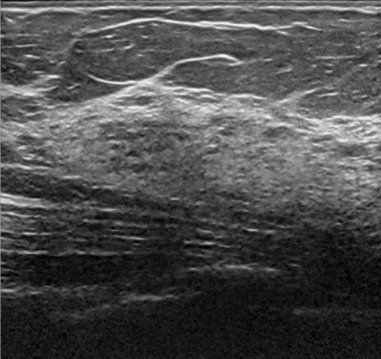
\includegraphics[height=.515\textheight]{sa1.png}
% \caption{ Breast US image example.}
% 		\end{figure}	
% \end{column}
% \end{columns}
% \end{frame}

\subsection{Image inspection to infer state of health}
%\subsection{Computer Aided Diagnosis (CAD)}

\begin{frame}\frametitle{State of health from image visual Inspection}
\setbeamercovered{transparent}
\begin{block}{Radiologic diagnosis error rates are similar to any other human visual inspection}
  \begin{itemize}
    \item Quality of the images.
    \item Ability to interpret the physical properties of the images.
  \end{itemize}
\end{block}
  \begin{enumerate}
    \item Double readings.
    \item Computer Aided Diagnosis(CAD).

  \end{enumerate}
\end{frame}


\begin{frame}\frametitle{BI-RADs Lexicon}
  \framesubtitle{A standardized toolkit tested for diagnosis}
  \footnotesize
  For each description section a single category is given based on some criteria
  \begin{itemize}
    \item \textbf{BKGD Echotexture :}
      \textit{Adipose, Fibro-Glandular or Heterogeneous}
      based on the visual texture present surrounding the lesion.
    \item \textbf{Mass shape :}
      \textit{Oval, Round, Irregular, Lobular}
      based on general shape of the lesion
    \item \textbf{Mass orientation :}
      \textit{Parallel, Non-Parallel}
      with respect to the general orientation of the skin layers
    \item \textbf{Mass margin :}
      \textit{Circumscribed, Indistinct, Angular, Microlobulated, Spiculated}
      based on the delineation of the lesion
    \item \textbf{Lesion boundary :}
      \textit{Abrupt interface, Echogenic halo}
      to differentiate when hyperechoic tissue surrounds the lesion
    \item \textbf{Echo pattern :}
      \textit{Anechoic, Hyperechoic, Complex, Isoechoic, Hypoechoic}
      based on the lesion appearance with respect to the adipose tissue
    \item \textbf{Posterior acoustic pattern :}
      \textit{Shadowing, Combined, Enhancement, No patter}
      based on how the background tissue posterior to the lesion is depicted
  \end{itemize}
\end{frame}

% \begin{frame}\frametitle{Take away}
%   \framesubtitle{Accurate delineations to develop CAD systems for BUS}
% \begin{figure}
% 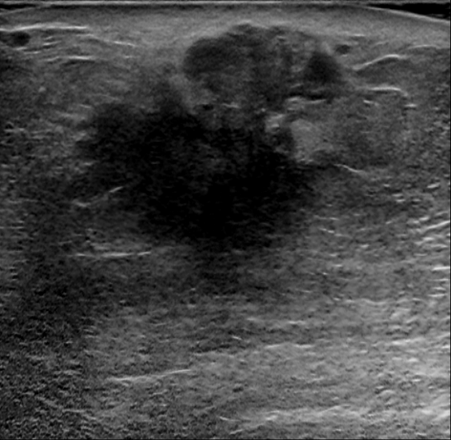
\includegraphics[trim=0 6 0 0,clip,height=.5\textheight]{a110105_094.png}~
% 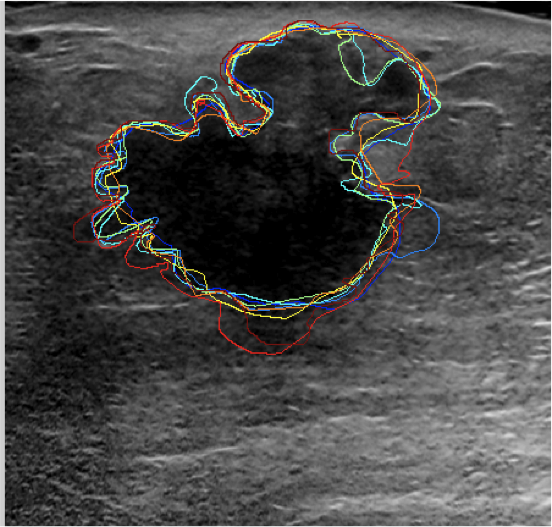
\includegraphics[trim=6 0 0 0,clip,height=.5\textheight]{segment.png}
% \end{figure}
% \end{frame}
